\documentclass[a4paper]{report}
\usepackage[utf8]{inputenc}
\usepackage[T1]{fontenc} 
\usepackage[francais]{babel}
\usepackage{graphicx}
\usepackage{geometry}
\usepackage{listings}
\usepackage{listingsutf8}
\usepackage{color}
\usepackage{fancyhdr}
\pagestyle{fancy}
\fancyhf{}
\lhead{2011/2012}
\rhead{IUT Nancy Charlemagne}
\geometry{hmargin=1cm,vmargin=2cm,lmargin=2cm,rmargin=2cm}
\lfoot{Mathieu LEROUX}
\cfoot{Projet tuteuré: Déduplication \\ Licence ASRALL}
\rfoot{\thepage}
\renewcommand{\footrulewidth}{2pt}
\lstset{
	language=bash,
	tabsize=2,
	extendedchars=true,
	commentstyle=\color{blue}
}
\begin{document}
	\chapter{Déduplication}
	La déduplication de données est une technique qui permet de minimiser de l'espace de stockage. Elle consiste à ne pas répliquer les données déja existantes sur le disque. Un fichier est décomposé sous forme de blocs de données car des fichiers peuvent avoir des blocs en commum. Le mécanisme de déduplication crée une table avec les index de tous les blocs de données des fichiers présents sur le disque. La taille des blocs peut varier selon les mécanismes utilisés mais plus les blocs sont petits, plus il y aura de chance qu'un autre bloc soit identique et donc, plus la déduplication sera efficace. En général, cette taille ne dépasse pas les 128ko.
 
 Quand un utilisateur dépose un fichier, le mécanisme crée ses index et regarde s'il n'y a pas des blocs déjà existants. Si des blocs sont similaires alors une simple référence aux blocs déjà existants sera crée. Le schéma ci-dessous montre comment la déduplication fonctionne. Les blocs étant de la même couleur sont considérés identiques.\\
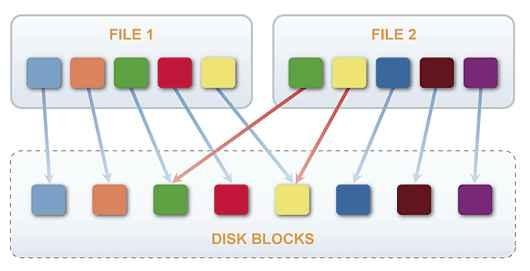
\includegraphics[width=10cm]{img/deduplication.jpg}

Il existe deux types de dépuplication: la déduplication à la volée (à la source) et la déduplication hors ligne (à la destination). La déduplication à la volée analyse les fichiers avant de les stocker pour savoir s'ils n'existent pas déjà sur le disque. Cette technique utilise une forte consommation CPU et mémoire. L'autre technique consiste à copier dans un premier temps le fichier sur le disque avant de tester s'il existe déjà. Cela nécessite de prévoir un espace de stockage tampon plus important. \\

Dans un contexte de serveur de messagerie et de fichiers centralisés, la déduplication de données peut très rapidement économiser de nombreux gigaoctets d'espace disque ainsi que la diminution de la bande passante qui aurait été utilisée pour la sauvegarde. En effet, dans le cas où un même mail de 1Mo est envoyé à cinquante destinataires alors l'économie du disque sera de 50-1 megaoctets (stockage d'un seul mail). La déduplication est faite pour des fichiers tels que des documents bureautiques ou des machines virtuelles qui ont souvent de nombreux blocs en commun.\\
Le terme inverse de la déduplication est la réhydratation. Elle fait appel à la table des index afin de renvoyer tous les blocs de données référencés pour un fichier demandé.\\

Certain outils comme LessFS permettent de dédupliquer et de compresser les blocs de données. Cela permet de gagner encore plus d'octets sur le disque mais nécessite une consommation mémoire et CPU plus importante.

	\chapter{ZFS}
	\section{Introduction}
	Le système de fichier ZFS (Zettabyte File System) a été conçu par Sun en 2005 et est sous licence CDDL.  Il n'était disponible que sous Solaris mais est devenu récemment disponible sous linux. Il est l'un des systèmes de fichiers les plus intéressants du marché. En effet, ZFS intègre de nombreux avantages que d'autres n'ont pas. Voici une liste de ses principaux avantages: \\
	\begin{itemize}
		 \item Pas de limites pratiques (taille des disques, fichiers, ...)
		 \item Garantir la sécurité des données (intégrité, disponibilité)
		 \item Administration simplifiée
		 \item Gestionnaire de volume intégré
		 \item Compression
		 \item Snapshot
		 \item Duplication
		 \item Quotas et réservation d’espace
		 \item Performances élevées
		 \item Indépendant de l’architecture matérielle\\
	\end{itemize}
	ZFS est un système de fichier 128 bits contrairement aux autres systèmes qui sont de 64 bits. Ainsi ses limites sont de 16 milliards de milliards fois plus autant dire qu'il n'a quasi pas de limite. Afin d'optimiser ses performances, ZFS utilise tout l'espace disponible de la RAM pour créer un énorme cache. Ce procédé s'appelle ARC (Adaptive replacement cache). Il peut poser problème aux autres processus qui testent la mémoire inutilisée avant de ce lancer mais cette mémoire est souvent inutilisée. Il peut être partagé via le réseau avec d'autres systèmes de fichiers comme nfs ou samba. Ainsi même depuis des systèmes qui ne le supporte pas, il sera accessible.\\
	\section{Stockage}
	ZFS fonctionne avec un pool. C'est un ensemble de périphériques qui fournissent de l’espace pour le stockage et la duplication des données comme le raid logiciel ou matériel. Traditionnellement, les systèmes de fichiers classiques étaient restreint à un périphérique par système. Avec la gestion des volumes, il est possible de créer plusieurs systèmes de fichiers sur un périphérique.\\
	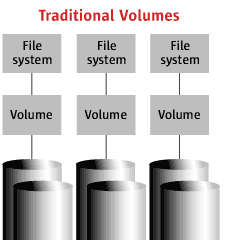
\includegraphics[width=5cm]{img/volumes_tradicionais.png}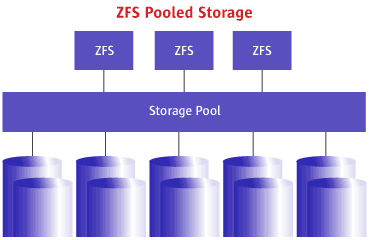
\includegraphics[width=7cm]{img/armazenamento_pooled_zfs.png}\\

	Voici les différentes unités de base de stockage de données :\\
	\begin{itemize}
		 \item Disques : entiers ou juste une partition
		 \item Fichiers dans un autre système de fichiers
		 \item Miroirs : 2 (ou plus) disques, partitions ou fichiers
		 \item Raid-z : plusieurs disques, variante de RAID-5\\
	\end{itemize}
	ZMirror est un miroir classique. Il utilise les mécanismes de checksum pour valider les lectures sur un composant et bascule sur le second s'il détecte une erreur puis corrige le composant défaillant (si possible). Le système Raid-z est similaire au procédé Raid 5. Il utilise les checksums (SHA-256 + fletcher) et repose sur le copy on write : supprime le "write-hole".
	\section{Garantir la sécurité des données (intégrité, disponibilité)}
		Avec ZFS, toutes les données et métadonnées sont vérifiées selon un algorithme de somme de contrôle. Lorsque qu'un bloc de données endommagé est détecté, ZFS recupère les données correctes à partir d'une autre copie redondante et répare les données endommagées en les remplaçant par celles de la copie.
	\section{Snapshots}
		Un snapshot (ou instantané) est une copie en lecture seul d'un système de fichier ou d'un volume. ZFS permet donc de pouvoir sauvegarder et restaurer l'image du volume désiré. La création d'un instantané est quasi immédiate. Les instantanés utilisent l'espace de stockage du pool. Une seul opération, dite atomique, permet de créer des instantanés récursifs au système désiré. Ils ne sont pas directement accessible mais peuvent etre clonés, sauvegardés ou restaurés. D'une manière simple et rapide, un instantané peut etre créé, restauré ou supprimé:
		\begin{lstlisting}[language=ksh,texcl]
			#creation du snapshot nommé "nomSnapshot" du système de fichier systèmeZFS au sein du pool "pool"
			zfs snapshot pool/systemeZFS@nomSnapshot
			#Opération atomique (récursif)
			zfs snapshot pool/systemeZFS@nomSnapshot 
			#Instantané "nomSnapshot" supprimé
			zfs destroy pool/systemeZFS@nomSnapshot 
			#Restauration de l'instantané "nomSnapshot"
			zfs rollback pool/systemeZFS@nomSnapshot 
			#Permet de voir les différences entre les deux instantanés
			zfs diff pool/systemeZFS@nomSnapshot pool/systemeZFS@nomSnapshot2 
		\end{lstlisting}
	\section{Clones}
		Un clone est un volume ou un système de fichiers accessible en écriture dont le contenu initiale est celui de l'instantané qu'il la créer. En effet, les clones ne sont créer que par des instantanés et une dépendance se crée entre les deux. Néanmoins, les clones n'héritent pas les propriétés de leur instantané mais peuvent être modifiés via les commandes zfs set et zfs get. Les commandes ci-dessous permettent de créer un snapshot et de l'utiliser pour créer un clone.
		\begin{lstlisting}[language=ksh,texcl]
			# creation du snapshot
			zfs snapshot pool/systemeZFS@nomSnapshot 
			# creation du système de fichier /home à l'aide du snapshot
			zfs clone pool/systemeZFS@nomSnapshot pool/home 
		\end{lstlisting}
	\section{Compression}
		La compression est une option de ZFS. Elle peut etre activer pour chaque systèmes de fichiers et snapshots via l'option compression. Ses valeurs sont soient on, off,lzjb (algorithme tiré de Lempel ziv), gzip et gzip-n. Son taux de compression sera d'environ de 2 suivant le type de données à compresser et l'option choisit. Exemples:
		\begin{lstlisting}[language=ksh,texcl]
			# pour le système de fichier
			zfs set compresison=on pool/systemeZFS 
			# pour le snapshot
			zfs set compression=on pool/systemeZFS@nomSnapshot 
		\end{lstlisting}
	\section{Quotas et reservation d'espace}
		ZFS permet de limiter la taille de stockage à un système de fichier via l'option "quota" et permet de réserver un espace à un système de fichier via l'option "reservation". Ces propriétés sont très intéréssantes quand il s'agit de limiter de l'espace disque à des utilisateurs. ZFS préconise de créer un système de fichiers par utilisateur qui serait monté au sein du même pool. Il est donc possible de créer des cotas par utilisateurs et par groupes via les options zfs userquotas et zfs groupquotas. Il sera possible de lister l'espace utilisé par utilisateur ou par groupe.Voici quelques exemple d'utilisations :
		\begin{lstlisting}[language=ksh,texcl]
			#attribution d'un quota de 10 gigaoctets au système de fichier mat
			zfs set quota=10G pool/home/mat 
			#attribution d'un quota de 10 gigaoctets à l'utilisateur mat
			zfs set userquota@mat=10G pool/home 
			#attribution de 100 gigaoctets au groupe etudiant
			zfs set groupquota@etudiant=100G pool/etudiant 
		\end{lstlisting}
	\chapter{Compression}
	Tout comme la déduplication, la compression est une technique qui permet d'économiser de l'espace de stockage. Chaque fichier est constitué d'une succession de millions de bits 0 ou 1. La compression permet de diminuer le nombre de bits que constitue un fichier en changeant la succession de bits de départ. Suivant l'algorithme de codage utilisé, le taux de compression peut différer. Les algorithmes d'encodage sont plus ou moins efficaces selon le type de fichier compressé.\\
 Il existe deux types de compression: la compression avec pertes et sans perte. La compression sans perte signifie qu'après la décompression, le fichier sera identique au fichier compressé. C'est le plus souvent utilisé sur des documents, des fichiers exécutables ou des archives. Ces données étant principalement des caractères texte, ils ne peuvent pas être modifiés. Les formats de documentation tels que txt, doc ou pdf sont donc compressés sans perte.  Tant qu'à la compression avec perte, les fichiers décompressés ne seront pas exactement identiques au fichier original mais les informations seront sensiblement les mêmes. Les types de fichiers utilisés par cette compression sont les images, les sons et les vidéos. Cett technique se repose sur la limitation des sens de l'homme comme la vision et l'audition. L'homme ne pourra donc pas identifier les différences entre le fichier original et le fichier après décompressage. Les formats de fichiers jpeg, avi ou mp3 sont donc compressés avec pertes. \\
Pour chaque technique de compression, il existe plusieurs algorithmes de codage.\\
	\section{Compression sans perte}
	Parmi les algorithmes sans perte, il y a les algorithmes tels que Lempei-Ziv ou le codage RLE (Run-Length Encoding) qui consistent à remplacer des suites de bits utilisées plusieurs fois dans un même fichier. D'autres algorithmes comme l'algorithme de codage Huffman détermine les suites de bits et plus une suite est utilisée souvent, plus la suite qui la remplacera sera courte.
	\subsection{L'algorithme Lempel-Ziv}
		Cet algorithme se divise en deux versions distinctes : LZ77 et LZ78. Ces algorithmes utilisent un dictionnaire où ils référencent les motifs récurrents. A la rencontre d'un motif du dictionnaire, une simple référence au motif est faite (fenêtre glissante). La déduplication utilise globalement le même procédé.\\
	\subsubsection{LZ77}
		La compression LZ77 encode avec un taux de compression inférieur à d'autres algorithmes comme PPM et CM (voir ci-dessous) mais a le double avantage d'être rapide et asymétrique. Cela lui permet d'utiliser un algorithme de décompression différent de celui de la compression. Ainsi, la compression pourra être rapide et la décompression performante. Les variantes LZSS et LZMA sont basées sur la compression LZ77 et supprime quelques inconvénients de celle-ci tels que le taux de compression assez faible (pour LZMA) ou le problème si aucun motif récurrent n'est rencontré (pour LZSS). Ce problème aura pour conséquence d'augmenter la taille du fichier. La compression LZ77 est la base des algorithmes comme Deflate (ZIP, gzip) et donc LZMA (7-zip).
	\subsubsection{LZ78}
		La compression LZ78 ou Lempel-Ziv-Welch utilise aussi un dictionnaire mais au lieu de le remplir au fur et à mesure des motifs rencontrés, il crée un dictionnaire initial de tous les symboles possibles. Cela permet d'améliorer la compression car les données du dictionnaire ne devant plus être envoyées au décompresseur, l'espace utilisé est réduit. L'utilisation de cette technique a été réduite jusque 2003 car elle a été brevetée par UNISYS qui n'avait pas laissé la licence libre.
	\subsubsection{LZO}
		Lempel-Ziv-Oberhumer (LZO) est un algorithme de compression en temps réel se basant sur les dictionnaires. Ces avantages sont une compression et décompression rapide. L'un des logiciels l'utilisant est lzop.
	\subsection{L'algorithme RLE}
		Le run-length encoding (codage par plages) est une technique de compression qui s'applique uniquement sur des documents scannés en noir et blanc tels que des fax. Elle consiste à factoriser les termes d'une même couleur. Ainsi la chaîne : NNNNNNNBBBBNNNNNNNNNNBB (N étant le nombre de points noirs et B étant le nombre de points blancs) sera encodée par RLE en : 7N4B10N2B . Les formats d'images utilisent cette compression en considérant que toutes les lignes de pixels sont jointes pour former une unique séquence de couleur. Les images BMP utilisent cette compression en 1,4 et 8 bits/pixel (noir et blanc, 16 couleurs et 256 couleurs). Le format PCX utilise aussi cette compression pour les images de 8 et 24 bits/pixels. Celles de 24 bits étant découpées en trois parties de 8 bits chacune.
	\subsection{Codage par modélisation de contexte}
	\subsubsection{Prédiction par reconnaissance partielle (PPM)}
		La prédiction par reconnaissance partielle se base sur une modélisation de contexte pour évaluer la probabilité des différents symboles. Le contexte est un ensemble de symboles déjà rencontrés dans la source de données. Elle utilise les données déjà analysées pour en déduire les données à analyser. Ainsi plus le contexte est long, meilleur sera la prédiction et donc la compression. La prédiction obtenue servira d'entrée à un codage entropique comme le codage Huffman. Elle a l'avantage d'être l'une des plus performantes sur la compression de fichiers texte mais a l'inconvénient de consommer énormément de mémoire si le contexte est très grand. La PPM est un algorithme symétrique contrairement à Lempel-Ziv ce qui signifie qu'il utilise le même pour la compression que pour la décompression. Cela implique un temps d'exécution identique et assez lent.
	\subsubsection{Pondération de contextes (CM)}
		La pondération de contextes consiste à utiliser plusieurs prédicteurs (par exemple des PPM) pour obtenir l'estimation la plus fiable possible du symbole à venir. A l'image de la prédiction par reconnaissance partielle, les taux de compressions sont très élevés mais proportionnellemnt aussi lents que la taille du contexte.
	\subsection{L'algorithme de codage Huffman}
		Cette compression s'apparente à la compression du code morse. Elle consiste donc à coder les séquences fréquentes sur peu de place et ce qui revient rarement sur des séquences plus longues. L'inconvénient avec ce procédé c'est qu'il faut avoir analysé tout le fichier pour créer une table avec les redondances avant de pouvoir le compresser. Il faut donc envoyer la table pour pouvoir le décompresser ce qui peut être problématique quand le fichier à compresser est petit. Le codage Huffman adaptatif corrige ce problème car il remplit au fur et à mesure la table et démarre la compression avec une table de base. \\
	Ce codage est utilisé en seconde compression après que le premier algorithme (tel que LZ77) est mis en évidence la redondance d'information. Ce codage peut être utilisé pour la compression tels que JPEG, MPEG ou MP3 où les données imperceptibles par l'homme sont supprimées mais on parle donc de compression avec pertes.
	\section{Compression avec pertes}
		La compression avec pertes s'utilisent donc sur des données perceptibles par l'homme comme les sons, les images ou les vidéos. Elles suppriment les données que l'homme ne perçoit pas ou quasiment pas. Ainsi pour le format JPEG 2000, la compression est de 1 bit/pixels au lieu de 24 bits/pixels. La compression avec pertes est une technique irréversible c'est à dire qu'il ne sera pas possible de retrouver le fichier original. Il existe trois grandes familles de compression avec pertes: la compression par prédiction, par transformation et la compression basée sur les récurrences fractales de motif.
	\subsection{Compression par prédiction}
		Cet algorithme repose sur un schéma de prédiction et un codage des erreurs entre la prédiction et le signal original. La prédiction consiste à prédire les données à venir en fonction des données analysées. Les erreurs étant souvent de faibles magnitudes, une compression intéressante est possible grâce à la diminution des bits nécessaires à l’opération. Certain formats de codecs de microsoft et d'Apple utilisent cette compression.
	\subsection{Compression par transformation}
		Cet algorithme transforme le signal en atténuant les fréquences non décelables par l'homme. Cette technique transforme donc le signal du domaine temporel au domaine fréquentiel afin de déterminer et de supprimer les pixels redondants.  Le schéma ci-dessous montre cette transformation.\\
	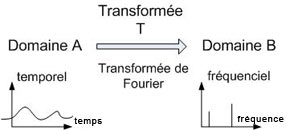
\includegraphics[width=5cm]{img/transformation.jpg} \\
La compression JPEG,JPEG 2000 ou encore MPEG utilise cette compression. Cette méthode de compression est la plus répandue au vue de ces performances.
	\subsubsection{La norme JPEG}
		La norme JPEG (Joint Photographic Experts Group) est une norme qui définit le format d'enregistrement et l'algorithme de décodage pour une représentation numérique compressée d'une image fixe. La norme JPEG peut être compressée sans perte mais son taux de compression n'est que de 2 au lieu de 3 à 100.
Le shéma ci-dessous montre ses étapes de compression et décompression.\\
		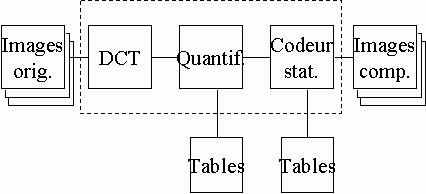
\includegraphics[width=10cm]{img/schema.jpg} \\
		Tout d'abord, le format JPEG commence par découper l'image en blocs de données comme beaucoup d'autres formats compressés avec pertes. Puis JPEG transforme les couleurs de chaque bloc à l'aide de la transformée DCT (transformée en cosinus discrète) assimilable à la transformée de Fourier qui transforme le signal temporel en signal fréquentiel (DCT). La valeur des fréquences résultantes détermineront leurs importances dans l'image. Une matrice de ces résultats sera générée. La quantification est l'étape qui permet de réduire considérablement la taille de l'image. En effet, elle utilise la DCT pour atténuer les fréquences non perceptibles par l'homme. La matrice résultante par la quantification sera ensuite codée par un algorithme RLE puis par un algorithme d'Huffman afin d'être compressée. Lors de la quantification et du codage, des tables sont créées et envoyées avec le fichier compressé pour la décompression.\\
	Lors de la compression du format JPEG sans perte, l'étape de la quantification n'est pas présente.

	\subsubsection{Compression par ondelette}
		La compression (ou transformée) par ondelette s'utilise globalement comme la norme JPEG mais génère une image de meilleure qualité avec un taux de compression supérieure (de 15 à 50). Contrairement à la transformée DCT, l'image est analysée plus finement et a un résultat plus proche de la perception humaine. Les codeurs JPEG 2000 et SPIHT utilisent tous deux une transformée en ondelettes dans leur schéma de compression. Les domaines d'utilisation de cette compression est l'imagerie médicale, les empreintes digitales ou encore dans le cinéma.

	\subsection{Compression basée sur les récurrences fractales de motif}
		La compression basée sur les récurrences fractales de motif aussi appelée compression fractale est utilisée pour la compression d'image. Son principe est de détecter les récurrences de motifs et de supprimer les informations redondantes de l'image. Plusieurs méthodes existent mais la plus connue est la méthode Jacquin. Deux étapes composent cette méthode. Dans un premier temps, deux segmentations sont réalisées: une segmentation de figure source et destination. Ensuite pour chaque figure Source, une figure destination est cherchée afin de créer un couple pour minimiser une erreur. Cette erreur est le résultat de leur soustraction après avoir dimensionné le couple de manière identique. A ce stade, des transformations comme la rotation peuvent être réalisées.
		
         \chapter{Mise en place d'un serveur de fichiers ZFS + NFS}
		Nous allons mettre en place un serveur de fichiers sur un système de fichiers ZFS pour les nombreux avantages cité ci-dessus. Il ne sera pas possible d'y ajouter des programmes de déduplication comme lessFS et openDedup car lessFS intègre un système de fichiers et Opendedup fonctionne avec SDFS. Néanmoins, le système de fichier intègre au même titre que la compression une propriété permettant la déduplication (présente uniquement sur Solaris). Il sera donc question de tester les principales fonctionnalités de ZFS comme la compression, l'intégrité des données (via raid-z), les sauvegardes (via les snapshots) et leurs restaurations. Je créerai ainsi 25 espaces utilisateurs de 1Go chacun où je stockerai divers types de fichiers comme des documents (.odt, .txt, .pdf), des images (jpeg, gif, png) et une base de données mysql. Afin de partager les systèmes de fichiers dédiés aux utilisateurs, ZFS permet d'activer le partage en nfs avec l'option sharenf à on.
	\section{Création des systèmes de fichiers}	
	 Nous allons créer un pool de stockage de 60Go en raidz2 qui est équivalent au raid 6. Pour ce faire, on utilisera sept fichiers de 10Go que nous allons créer par la commande ci-dessous :
		\begin{lstlisting}
			for i in `seq 0 6`;
			do dd if=/dev/zero of=./disque_$i bs=1M count=10000;
			done;
		\end{lstlisting}
	Parmi les sept fichiers utilisés, un sera utilisé pour les redondances d'informations du au raidz2. Ensuite, nous allons créer un pool de stockage nommé poolAsrall à l'aide de ces fichiers où seront installer les systèmes de fichiers. Le pool sera installé dans /media/. Voici la commande :
		\begin{lstlisting}
			zpool create poolAsrall raidz2 /media/Windows7/disque_{0,1,2,3,4,5,6} -m /media/poolAsrall
		\end{lstlisting}
	Puis on va créer un système de fichier /home/ au sein de ce pool et les cinquantes systèmes de fichiers dédiés aux utilisateurs.
		\begin{lstlisting}
			zfs create poolAsrall/home
			for i in `seq 0 49`;
			do zfs create poolAsrall/home/util_$i;
			done;
		\end{lstlisting}
	Afin de tester la compression de ses systèmes de fichiers, nous allons activer l'option qui sera récursive à tout ses sous systèmes de fichiers. Nous allons tester l'option on, off, lzjb, gzip, gzip-1, gzip-9 pour tout les espaces utilisateurs.
		\begin{lstlisting}
			zfs set compression=on poolAsrall/home
		\end{lstlisting}
	Puis on va les remplir de 1,42Go de fichiers divers et variés. Pour cela, nous avons copié le contenu de notre dossier Documents qui fait cette taille et qui contient:
		\begin{itemize}
			\item 40 pourcents de fichiers textes (sh, php, html, txt,..)
			\item 30 pourcents d'images (png, gif, jpeg)
			\item 15 pourcents de pdf
			\item 15 pourcents d'autres types de fichiers
		\end{itemize}
	Par le script suivant, nous allons remplir ces espaces utilisateurs.
		\begin{lstlisting}
			for i in `seq 0 24`;
			do cp -R  /home/mathieu/Documents poolAsrall/home/util_$i;
			done;
		\end{lstlisting}
	Concernant la base de données mysql, il faut changer le repertoire de stockage des données dans le fichier /etc/mysql/my.conf puis copier le dossier /var/lib/mysql et le coller dans le dossier où nous voulons stocker les données. L'essentiel est de garder les droits du dossier original. \\
Dans notre test, nous allons créer un système de fichier bin puis mysql où allons stocker les données de la base.
		\begin{lstlisting}
			zfs create poolAsrall/bin
			zfs create poolAsrall/bin/mysql
			cp -a /var/lib/mysql /media/poolAsrall/bin/mysql
			cd /media/poolAsrall/bin/mysql && tar -xvf mysql.tgz
		\end{lstlisting}
	\section{Etat du système}
	Nous allons visualiser l'etat du système mise en place. Pour commencer, nous allons regarder l'etat du pool.
		\begin{lstlisting}
			zpool status
		\end{lstlisting}
		\begin{lstlisting}[backgroundcolor=\color{yellow}]
			pool: poolAsrall
			 state: ONLINE
			 scrub: none requested
			config:

				NAME                          STATE     READ WRITE CKSUM
				poolAsrall                    ONLINE       0     0     0
				  raidz2                      ONLINE       0     0     0
				    /media/Windows7/disque_0  ONLINE       0     0     0
				    /media/Windows7/disque_1  ONLINE       0     0     0
				    /media/Windows7/disque_2  ONLINE       0     0     0
				    /media/Windows7/disque_3  ONLINE       0     0     0
				    /media/Windows7/disque_4  ONLINE       0     0     0
				    /media/Windows7/disque_5  ONLINE       0     0     0
				    /media/Windows7/disque_6  ONLINE       0     0     0

			errors: No known data errors
		\end{lstlisting}
		Les disques créés étant situés dans ma partition dédiée à Windows. Par la commande ci-dessous, on peut visualiser l'espace utilisé et libre du pool. Comme aucun quota ou reservation n'a été précisé, les systèmes de fichiers créés à l'interieur du pool utiliserons tous son espace jusqu'à saturation.
		\begin{lstlisting}
			zpool list
		\end{lstlisting}
		\begin{lstlisting}[backgroundcolor=\color{yellow}]
			NAME         SIZE   USED  AVAIL    CAP  HEALTH  ALTROOT
			poolAsrall    68G  48,8G  19,2G    71%  ONLINE  -
		\end{lstlisting}
	\subsection{Schéma de l'installation}
		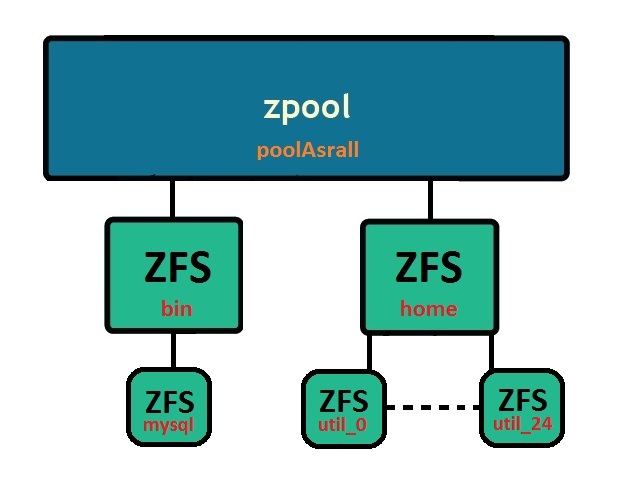
\includegraphics[width=10cm]{img/shema.jpg}\\
	Nous allons visualiser l'espace utilisé par chaque système de fichiers.
		\begin{lstlisting}
			df -h
		\end{lstlisting}
		\begin{lstlisting}[backgroundcolor=\color{yellow}]
			Sys de fichiers      Tail.  Occ. Disp. Occ. Monte sur
			/dev/sda7              54G   34G   18G  66% /
			none                  1,5G  332K  1,5G   1% /dev
			none                  1,5G  116K  1,5G   1% /dev/shm
			none                  1,5G  244K  1,5G   1% /var/run
			none                  1,5G     0  1,5G   0% /var/lock
			none                  1,5G     0  1,5G   0% /lib/init/rw
			none                   54G   34G   18G  66% /var/lib/ureadahead/debugfs
			/dev/sda2             187G  149G   39G  80% /media/Windows7
			/dev/sda5             1,1G  149M  892M  15% /media/b07f0352-66e0-4503-ad13-9c0524b40293
			poolAsrall             13G   49K   13G   1% /media/poolAsrall
			poolAsrall/home        13G  102K   13G   1% /media/poolAsrall/home
			poolAsrall/bin         13G   22M   13G   1% /media/poolAsrall/bin
			poolAsrall/bin/mysql   13G   22M   13G   1% /media/poolAsrall/bin/mysql
			poolAsrall/home/util_0
					       15G  1,4G   13G  10% /media/poolAsrall/home/util_0
			poolAsrall/home/util_1
					       15G  1,4G   13G  10% /media/poolAsrall/home/util_1
			poolAsrall/home/util_2
					       15G  1,4G   13G  10% /media/poolAsrall/home/util_2
			poolAsrall/home/util_3
					       15G  1,4G   13G  10% /media/poolAsrall/home/util_3
			poolAsrall/home/util_4
					       15G  1,5G   13G  10% /media/poolAsrall/home/util_4
			poolAsrall/home/util_5
					       15G  1,5G   13G  10% /media/poolAsrall/home/util_5
			poolAsrall/home/util_6
					       15G  1,5G   13G  10% /media/poolAsrall/home/util_6
			poolAsrall/home/util_7
					       15G  1,5G   13G  10% /media/poolAsrall/home/util_7
			poolAsrall/home/util_8
					       15G  1,5G   13G  10% /media/poolAsrall/home/util_8
			poolAsrall/home/util_9
					       15G  1,4G   13G  10% /media/poolAsrall/home/util_9
			poolAsrall/home/util_10
					       15G  1,4G   13G  10% /media/poolAsrall/home/util_10
			poolAsrall/home/util_11
					       15G  1,4G   13G  10% /media/poolAsrall/home/util_11
			poolAsrall/home/util_12
					       15G  1,4G   13G  10% /media/poolAsrall/home/util_12
			poolAsrall/home/util_13
					       15G  1,4G   13G  10% /media/poolAsrall/home/util_13
			poolAsrall/home/util_14
					       15G  1,4G   13G  10% /media/poolAsrall/home/util_14
			poolAsrall/home/util_15
					       15G  1,4G   13G  10% /media/poolAsrall/home/util_15
			poolAsrall/home/util_16
					       15G  1,4G   13G  10% /media/poolAsrall/home/util_16
			poolAsrall/home/util_17
					       15G  1,4G   13G  10% /media/poolAsrall/home/util_17
			poolAsrall/home/util_18
					       15G  1,4G   13G  10% /media/poolAsrall/home/util_18
			poolAsrall/home/util_19
					       15G  1,4G   13G  10% /media/poolAsrall/home/util_19
			poolAsrall/home/util_20
					       15G  1,4G   13G  10% /media/poolAsrall/home/util_20
			poolAsrall/home/util_21
					       15G  1,4G   13G  10% /media/poolAsrall/home/util_21
			poolAsrall/home/util_22
					       15G  1,4G   13G  10% /media/poolAsrall/home/util_22
			poolAsrall/home/util_23
					       15G  1,4G   13G  10% /media/poolAsrall/home/util_23
			poolAsrall/home/util_24
					       15G  1,4G   13G  10% /media/poolAsrall/home/util_24
			/dev/sda3             125G  116G  8,5G  94% /media/Data

		\end{lstlisting}
		\subsection{Compression}
			Les tests sur les différentes compressions ont été fait de cette manière:
			\begin{itemize}
				\item poolAsrall/home/util\_0 - 3 -> compression On : 1,39Go
				\item poolAsrall/home/util\_4 - 8 -> compression Off : 1,42Go
				\item poolAsrall/home/util\_9 - 13 -> compression lzjb : 1,40Go
				\item poolAsrall/home/util\_14 - 18 -> compression gzip : 1,36Go
				\item poolAsrall/home/util\_19 - 21 -> compression gzip-1 : 1,37Go
				\item poolAsrall/home/util\_22 - 24 -> compression gzip-9 : 1,36Go \\
			\end{itemize}
			Nous pouvons constater que la compression à la volée du système de fichiers ZFS permet de gagner environ quatre pourcents grâce à l'algorithme de compression gzip. En effet, contrairement à l'algorithme lzjb qui est tiré de Lempel ziv, gzip compresse grâce à Lempel ziv et Deflate. Le taux de compression peut paraitre assez faible mais ce gain de place sera beaucoup plus élevé sur du contenu textes. De plus, la compression est juste une option parmi les nombreuses que compte ZFS. Malheureusement, la consommation mémoire qui est très élevé pose des problèmes lors du rédémarrage qui parfois, ne réussi à monter tout les systèmes fautes de places mémoires.
		\subsection{Snapshots et restaurations de ZFS}
			Sous ZFS, il est possible de faire des snapshots sur tous les systèmes de fichiers d'un pool. Ainsi, il sera possible de sauvegarder séparément les systèmes de fichiers récursivement avec leurs fils ou non. Leurs restaurations se feront elles aussi de manière individuelle. Après avoir réaliser le snapshot désirer, il sera judicieux d'envoyer la sauvegarde sur un support sécurisé. Afin de restaurer la sauvegarde réalisée, il faudra supprimer ce système de fichiers puis le restaurer par la commande "zfs receive". Nous allons réaliser un snapshot du système de fichier mysql, le supprimer et le restaurer par les commandes suivantes:
		\begin{lstlisting}[language=ksh,texcl]
			# Création du snapshot
			zfs snapshot poolAsrall/bin/mysql@snapMysql.snap
			# Sauvegarde du snapshot
			zfs send poolAsrall/bin/mysql@snapMysql.snap > /home/mathieu/Documents/snapMysql.snap
			# Suppression du système de fichier poolAsrall/bin/mysql
			zfs destroy poolAsrall/bin/mysql
			# Restauration de la sauvegarde
			zfs receive poolAsrall/bin/mysql < /home/mathieu/Documents/snapMysql.snap
			# Changement du point de montage car celui par défaut sera son nom
			zfs mountpoint=/media/poolAsrall/bin/mysql poolAsrall/bin/mysql 
		\end{lstlisting}
		
		Après m'être connecter à une base de données mysql nommé wiki, j'ai créé et sauvegardé un snapshot du système poolAsrall/bin/mysql qui contenait les données de mysql. La sauvegarde ayant pour nom snapMysql.snap, et aura la même taille que le système de fichier sauvegardé. Après avoir supprimé ce système, je l'ai donc restaurer via la sauvegarde. La connexion à cette base se refait parfaitement, ainsi que l'accés à ces données. \\
		Nous allons tester la sauvegarde incrémentale de zfs en insérant une ligne dans la base wiki et en comparant avec l'ancien snapshot :\\
		\begin{lstlisting}[language=ksh,texcl]
			# Ajout d'une ligne dans la base mysql "wiki"
			# Création du second snapshot
			zfs snapshot poolAsrall/bin/mysql@snapMysql2.snap
			# Enregistrement de la difference entre les deux snapshots
			zfs send -i poolAsrall/bin/mysql@snapMysql.snap poolAsrall/bin/mysql@snapMysql2.snap > diff.snap
			# Taille du snapShot snapMysql.snap soit 42Mo
			ls -ali snapMysql.snap
		\end{lstlisting}
		\begin{lstlisting}[backgroundcolor=\color{yellow}]
			1591678 -rw-r--r-- 1 root root 44766176 2012-03-11 16:53 ../snapMysql.snap
		\end{lstlisting}
		\begin{lstlisting}[language=ksh,texcl]
			# Taille de l'incrément diff.snap soit 1.1Mo
			ls -ali diff.snap
		\end{lstlisting}
		\begin{lstlisting}[backgroundcolor=\color{yellow}]
			1582651 -rw-r--r-- 1 root root 1137672 2012-03-12 22:23 diff.snap
		\end{lstlisting}
		Comme précédemment, nous allons supprimer le système de fichier poolAsrall/bin/mysql avant de pouvoir le restaurer via le snapShot et l'incrément. Avant de pouvoir restaurer un incrément, il faut d'abord réaliser un rollback depuis le snapshot. La commande zfs rollback permet, comme son nom l'indique, de retourner aux données d'un snapshot donné.
		\begin{lstlisting}[language=ksh,texcl]
			# Destruction du système de fichier
			zfs destroy poolAsrall/bin/mysql
			# Restauration du snapshot
			zfs receive poolAsrall/bin/mysql < /home/mathieu/Documents/snapMysql.snap
			# Retour au snapshot
			zfs rollback poolAsrall/bin/mysql@snapMysql.snap
			# Insertion de l'increment au système
			zfs receive poolAsrall/bin/mysql < diff.snap
		\end{lstlisting}
		Concernant les sauvegardes à chauds, la restauration posera des problèmes si une modification de la base est en cours. Afin de corriger ce problème, il faudra utiliser les commandes de mysql lock et unlock avant et après le snapshot.
		\subsection{Rsnapshot}
		\subsubsection{Introduction}
		Rsnapshot est un logiciel libre qui permet de réaliser des sauvegardes et restaurations. Ces sauvegardes sont incrémentales: si elles sont réalisées tout les jours et qu'elles contiennent des fichiers identiques alors des liens en durs seront fait de cette sauvegarde à la sauvegarde précédente. Le nom des sauvegardes auront le noms de l'option de l'intervalle (hourly.x, daily.x, monthly.x et yearly.x) avec x le numéro de la sauvegarde. La sauveagrde la plus récente portant le numéro 0, et dès qu'une nouvelle sauvegarde sera réalisée alors la sauvegarde 0 deviendra 1 et ainsi de suite. 
		\subsubsection{Installation et configuration}
		On peut l'installer via le gestionnaire de paquet:
		\begin{lstlisting}
			sudo apt-get install rsnapshot
		\end{lstlisting}
		Rsnapshot n'a qu'un fichier de configuration /etc/rsnapshot.conf où est précisé le répertoire de destination des sauvegardes, les emplacements à sauvegarder, les scripts à éxécuter ou la périodicité des sauvegardes à éxécuter. Rsnapshot n'a pas prévu un traitement spécifique pour la sauvegarde des bases de données. Ainsi, il utilise les programmes propres aux sauvegardes de bases de données comme pg\_dumpall pour postgresql et mysqldump pour mysql. Des scripts pour l'utilisation de ces programmes sont mis à disposition dans un des dossiers sources de rsnapshot. Ils contiennent deux lignes: l'une pour utiliser le programme propre de sauvegarde de la base de données et l'autres pour changer les droits du fichier résultant. Dans mon cas, je vais donc sauvegarder ma base mysql via ce script. Voici les principales configurations du fichier rsnapshot.conf .
		\begin{lstlisting}[language=ksh,texcl]
			# Spécification du répertoire de destination des sauvegardes
			snapshot_root   /home/mathieu/.snapshots/
			#Pour utiliser les sauvegardes via ssh
			cmd_ssh        /path/to/ssh
			# Spécification de l'intervalles des sauvegardes
			interval        hourly  6
			interval        daily   7
			# Spécification du repertoire à sauvegarder et de l'emplacement dans le repertoire de destination
			backup  /media/poolAsrall/home/util_0           localhost/home/
			# Spécification du script à executer et de l'emplacement dans le repertoire de destination
			backup_script /usr/local/bin/backup_mysql.sh localhost/mysql/
		\end{lstlisting}
		\subsubsection{Sauvegardes}
		Afin d'automatiser la sauvegarde, il faudra ajouter le lancement de rsnapshot dans le cron. Dans l'exemple suivant, une sauvegarde est réalisée toutes les 4h et tout les jours à 23h.
		\begin{lstlisting}
			crontab -e
		\end{lstlisting}
		\begin{lstlisting}[backgroundcolor=\color{yellow}]
			0 */4 * * * /usr/local/bin/rsnapshot hourly
			30 23 * * * /usr/local/bin/rsnapshot daily
		\end{lstlisting}
		Pour tester rsnapshot, nous avons éxécuter la commande "/usr/bin/rsnapshot hourly" trois fois de suite. La première fois, la sauvegarde mettra quelques dizaines de secondes à se terminer alors que les sauvegardes suivantes ne mettrons que deux à trois secondes. Pourtant, la taille des dossiers créés sera la même. En effet, les dossiers sauvegardés n'étant pas modifier entre les sauvegardes, juste des liens en durs seront éffectuer de la première sauvegarde aux suivantes.
		\begin{lstlisting}[texcl]
			# on test l'espace utilisé par le dossier de sauvegarde .snapshots/
			du -hs .snapshots/
		\end{lstlisting}
		\begin{lstlisting}[backgroundcolor=\color{yellow}]
			1,5G	.snapshots/
		\end{lstlisting}
		La taille du dossier de l'espace utilisateur util\_0 de ZFS fait toujours 1,42Go. On peux constater que l'espace du dossier .snapshots/ est lègerement plus volumineux car il contient aussi la sauvegarde des bases mysql. Voyons le contenu de ce dossier et l'espace utilisé pour chacun des sous-dossiers hourly.
		\begin{lstlisting}
			du -hs .snapshots/*
		\end{lstlisting}
		\begin{lstlisting}[backgroundcolor=\color{yellow}]
			1,5G	./hourly.0
			868K	./hourly.1
			868K	./hourly.2
		\end{lstlisting}
		Comme on peux le constater, l'espace de la sauvegarde la plus récente contient les données et les anciennes sauvegardes font justes des liens vers ces fichiers. A chaque modification d'un de ses fichiers, la réécriture du fichier devrait etre effectué. Nous allons copié un fichier iso de 417Mo dans le repertoire util\_0, réalisé une sauvegarde, supprimer ce fichier et réaliser une nouvelle sauvegarde.
		\begin{lstlisting}
			du -ms .snapshots/*
		\end{lstlisting}
		\begin{lstlisting}[backgroundcolor=\color{yellow}]
			1481	.snapshots/hourly.0
			417	.snapshots/hourly.1
			1	.snapshots/hourly.2
			1	.snapshots/hourly.3
		\end{lstlisting}
		On peux constater que l'or de la modification du repertoire à sauvegarder, Rsnapshot rajoute le fichier entier au snapshot. Puis si le fichier est toujours présent alors il réalisera juste un lien vers le snapshot qui contient ce fichier. Maintenant, nous allons tester si Rsnapshot analyse juste la derniere sauvegarde ou toutes les sauvegardes pour voir si des fichiers existent déja afin de réaliser les liens. Pour ce faire on va réaliser une sauvegarde, le rajout du même fichier de 417Mo puis une nouvelle sauvegarde. En testant la taille des dossiers, on verra si le fichier apparait une ou deux fois.
		\begin{lstlisting}
			du -ms .snapshots/*
		\end{lstlisting}
		\begin{lstlisting}[backgroundcolor=\color{yellow}]
			1897	.snapshots/hourly.0
			1	.snapshots/hourly.1
			417	.snapshots/hourly.2
			1	.snapshots/hourly.3
			1	.snapshots/hourly.4
		\end{lstlisting}
		Comme on peut le voir ci-dessus, le fichier entier de 417Mo apparait deux fois dans les snapshots. On peut donc en conclure que Rsnapshot compare juste le dossier à sauvegarder au dernier snapshot réalisé.
		\subsubsection{Restaurations}
			Avec rsnapshot, il n'y a pas de façon automatique incorporé pour restaurer des fichiers ou des bases de données. Il faudra donc effectuer les restauration manuellement en se déplaçant dans l'arborescence des sauvegardes et puis, en choisissant le ou les fichiers à restaurer. Afin de partager les sauvegardes avec NFS, il faudra créer un repertoire de sauvegarde propres à chaque utilisateur avec des droits de lecture où ils pourront choisir leurs fichiers sans les modifier,et les rapatrier à l'emplacement désiré. Concernant les bases de données, on pourra les restaurer en utilisant, de la meme manière que pour leurs sauvegardes, les programmes propres aux SGBD.
	\chapter{Déduplication avec LessFS}
		\section{Introduction}
		LessFS est un système de fichier permettant la déduplication.Lessfs s'utilise avec le logiciel FUSE (Filesystem in Userspace) et Tokyocabinet (jeu de librairie permettant d'utiliser une base de données). Contrairement au système de fichier normal comme ext3, lessfs stock uniquement les blocks de données qui n'existent pas déja. Quand un block de données existent déja, il fait une simple référence à ce fichier et stock cette référence dans les tables de TokyoCabinet.
		\section{Tests}
			Afin de tester lessfs sur un cas concret, nous avons choisit de mettre en place ce logiciel sur les données générées par un serveur mail. Ces données étant des fichiers textes, la déduplication devrait atteindre son maximum. La taille des données non dédupliqué du serveur mail est de 20Go. Dans un premier temps, tout les mails sont stockés dans des fichiers différents. Par défaut la taille des blocks de données générer par lessfs est de 128ko (le maximum). Nous allons donc tester avec cette taille de blocks puis avec une taille de blocks de 64ko et pour finir une taille de 4ko (le minimum). Plus la taille des blocks est faible, plus la déduplication devrait etre élevé car il y aura plus de chances de trouver un block identique mais cela générera énormement d'entrées/sorties et donc de consommation mémoire et CPU. Lessfs a un fichier de configuration où on précise le repertoire pour stocker les blocks de données, la base de données tokyocabinet, la taille du cache ou la taille des blocks (voir en annexe). Aussi, lessfs permet de compresser ces blocks de données. Les algorithmes possibles sont qlz (par défaut), qlz15, snappy, Deflate, bzip et lzo. Nous allons tester l'algorithme qlz, bzip, lzo et Deflate. Après avoir copié les données du serveur mail dans le système de fichier lessfs monté sur /media/lessfs. \\
			\begin{lstlisting}
				du -hs /media/lessfs/
			\end{lstlisting}
			\begin{lstlisting}[backgroundcolor=\color{yellow}]
				20G	/media/lessfs/
			\end{lstlisting}
			On constate que le repertoire fait bien une taille de 20 Go. Regardons maintenant la taille des repertoires stockant les blocks de données et la base de données. Celle ci devrait etre très largement inférieur. J'ai choisit de stocker ces données dans /data/, les blocks de données dans /data/dta/ et la base de données dans /data/mta.\\
		\subsection{Taille des blocks=4ko et Compression=qlz}
			\begin{lstlisting}
				du -hs /data/*
			\end{lstlisting}
			\begin{lstlisting}[backgroundcolor=\color{yellow}]
				11G	/data/dta
				694M	/data/mta
			\end{lstlisting}
			On peux constater que la déduplication a pas très bien fonctionner. Le nombre de blocks stockés dans la base est très important du aux très grand nombres de blocks a référencé. Le taux de déduplication est inférieur à deux et cela a mis 4h10 pour copier tout le contenu.\\

		\subsection{Taille des blocks=4ko et Compression=bzip}
			\begin{lstlisting}
				du -hs /data/*
			\end{lstlisting}
			\begin{lstlisting}[backgroundcolor=\color{yellow}]
				8,4G	/data/dta
				509M	/data/mta
			\end{lstlisting}
			La déduplication fonctionne légerement mieux que le test avec la compression qlz mais le temps reste très important. Cela a mis 3h30.
		\subsection{Taille des blocks=4ko et Compression=lzo}
			\begin{lstlisting}
				du -hs /data/*
			\end{lstlisting}
			\begin{lstlisting}[backgroundcolor=\color{yellow}]
				9,3G	/data/dta
				559M	/data/mta
			\end{lstlisting}
			Comme dans le test précédent, la déduplication est faible mais le temps imparti est très largement inférieur. Cela a mis 1h49.
		\subsection{Taille des blocks=4ko et Compression=Deflate}
			\begin{lstlisting}
				du -hs /data/*
			\end{lstlisting}
			\begin{lstlisting}[backgroundcolor=\color{yellow}]
				7,8G	/data/dta
				559M	/data/mta
			\end{lstlisting}
			La déduplication est légerement supérieur et cela mis un temps a peu près identique, c'est à dire 1h51.
		\subsection{Taille des blocks=64ko et Compression=qlz}
			\begin{lstlisting}
				du -hs /data/*
			\end{lstlisting}
			\begin{lstlisting}[backgroundcolor=\color{yellow}]
				2,4G	/data/dta
				99M	/data/mta
			\end{lstlisting}
				Avec la taille des blocks de 64ko, la déduplication est très largement supérieur et dans un temps lui aussi largement inférieur, c'est à dire 18 minutes. On constate aussi que la taille de la base de données est lui aussi inférieur car le nombre de blocks a référencé est moins important.
		\subsection{Taille des blocks=64ko et Compression=bzip}
			\begin{lstlisting}
				du -hs /data/*
			\end{lstlisting}
			\begin{lstlisting}[backgroundcolor=\color{yellow}]
				2,5G	/data/dta
				99M	/data/mta
			\end{lstlisting}
			Cette fois, la taux de deduplication est quasiment identique avec 8x mais cela a mis plus de deux fois plus de temps, c'est à dire 35 minutes. La compression bzip est donc bien moins rapide que qlz.
		\subsection{Taille des blocks=64ko et Compression=lzo}
			\begin{lstlisting}
				du -hs /data/*
			\end{lstlisting}
			\begin{lstlisting}[backgroundcolor=\color{yellow}]
			5,6G	/data/dta
			99M	/data/mta
			\end{lstlisting}
				La déduplication avec lzo est moins performante que celle avec bzip ou qlz mais elle se termine dans un temps largement inférieur, c'est à dire 19 minutes.\\
		\subsection{Taille des blocks=64ko et Compression=Deflate}
			\begin{lstlisting}
				du -hs /data/*
			\end{lstlisting}
			\begin{lstlisting}[backgroundcolor=\color{yellow}]
				1,7G	/data/dta
				99M	/data/mta		
			\end{lstlisting}
			Comme dans le test avec les blocks a 4ko, la compression la plus performante est Deflate. Dans ce cas, la compression a très bien fonctionné car elle a mis que 18 minutes avec un taux de 11,7.\\
		\subsection{Taille des blocks=128ko et Compression=qlz}
			
			\begin{lstlisting}
				du -hs /data/*
			\end{lstlisting}
			\begin{lstlisting}[backgroundcolor=\color{yellow}]
				1,7G	/data/dta
				84M	/data/mta
			\end{lstlisting}
			La taille de blocks deux fois supérieur, la déduplication et la compression avec qlz ont atteint les performances de la compression Deflate du test précédent. Malgré le taux de déduplication égale, le temps quand a lui, a mis 32 minutes.

		\subsection{Taille des blocks=128ko et Compression=bzip}
			\begin{lstlisting}
				du -hs /data/*
			\end{lstlisting}
			\begin{lstlisting}[backgroundcolor=\color{yellow}]
				1,6G	/data/dta
				84M	/data/mta
			\end{lstlisting}
			 Cette fois, la déduplication a bien fonctionné meme mieux que le premier test. La compression avec bzip fonctionne donc mieux que la compression qlz. Le taux de déduplication est de 12,5x en 36 minutes.\\

		\subsection{Taille des blocks=128ko et Compression=lzo}
		\begin{lstlisting}
			du -hs /data/*
		\end{lstlisting}
		\begin{lstlisting}[backgroundcolor=\color{yellow}]
			5,7G	/data/dta
			84M	/data/mta
		\end{lstlisting}
			Dans ce test le taux de déduplication n'est que 3.5x mais la compression lzo se rattrape dans la rapidité car le temps n'a été que de 19 minutes. Ce temps a été plus rapide que sur le système de fichier ext3 non dédupliqué.\\

		\subsection{Taille des blocks=128ko et Compression=Deflate}
			\begin{lstlisting}
				du -hs /data/*
			\end{lstlisting}
			\begin{lstlisting}[backgroundcolor=\color{yellow}]
				1,3G	/data/dta
				84M	/data/mta
			\end{lstlisting}
			On constate que la déduplication par Deflate est la plus performante car elle atteind un taux de 15.3x. De plus, la copie a mis un temps de 17 minutes.\\
		\subsection{Tableau récapitulatif}
			\begin{tabular}{|c|c|c|c|c|}
			  \hline
			  Taille des blocks / Compression & qlz & bzip & lzo & Deflate\\
			  \hline
			  4Ko & 1.8x/4h10 & 2,4x/3h30 & 2.15x/1h49 & 2.56x/1h51 \\
			  \hline
			  64Ko & 8.5x/18m & 8x/35m & 3.5x/19m & 11.7x/18m \\
			  \hline
			  128Ko & 11.7x/32m & 12.5x/36m & 3.5x/19m & 15.3x/17m\\ 
			   \hline
			\end{tabular}\\\\
			La déduplication avec lessFs est donc très performante mais cette performance est très liées aux performances de la machine l'utilisant. En théorie, on pouvait pensé que plus la taille des blocks était faible, plus lessFs pourrait trouvé des blocks similaires. Mais on a pu constater que dans le cas d'un serveur mail et d'une machine assez peu performante, la déduplication était la meilleure quand la taille des blocks était la plus élevé. Un test a été éffectué pour savoir le temps que mettait la copie du meme contenu sur un système de fichier ext3 non dédupliqué et le résultat a été de 23 minutes. LessFs est donc plus rapide de 6 minutes tout en diminiant la taille de plus de quinze fois. Parmi les différents tests, la compression avec Deflate a été la plus élevé car cette compression utilise l'algorithme LZ77 et le codage Huffman qui, sur du contenu qui revient souvent comme sur des mails est très performant. Si on désire sauvegarder ces donneés, c'est possible de "geler" la base tokyocabinet via une connexion telnet afin de réaliser une sauvegarde et une autre option permet de la "dégeler". Après l'avoir tester avec Rsnapshot, la restauration et l'accés aux données se réalise sans problème quand aucune écriture n'est en cours. Dans le cas contraire, la restauration s'effectuera sans problème mais aucun fichier ne sera accéssible. Les données seront donc corrompues.\\\\

			Testons maintenant une architecture du serveur mail différente. Cette fois, les mails de chaque utilisateur sont stockées dans un fichier. Il y aura donc un fichier par utilisateur mais les données seront identiques.

			\subsection{Taille des blocks=128ko et Compression=Deflate}
			\begin{lstlisting}
				du -hs /data/*
			\end{lstlisting}
			\begin{lstlisting}[backgroundcolor=\color{yellow}]
				2,0G	/data/dta
				83M	/data/mta
			\end{lstlisting}
			\subsection{Taille des blocks=4ko et Compression=Deflate}
			\begin{lstlisting}
				du -hs /data/*
			\end{lstlisting}
			\begin{lstlisting}[backgroundcolor=\color{yellow}]
				14G	/data/dta
				695M	/data/mta
			\end{lstlisting}
			
			Les performances avec lessFs peuvent donc varier suivant le nombre de fichier a traité malgré des données identiques mais misent sous une forme différentes. La déduplication a moins bien fonctionnée. Il a dédupliqué environ deux fois moins mais dans un temps lui aussi deux fois moins pour des blocks d'une taille de 128ko. Pour l'autre test, le temps a mit exactement la meme durée et la déduplication a été aussi deux fois moins performante. LessFS crée un fichier de stat dans le lequel il écrit le ratio de compression qu'il a réalisé sur chaque fichier (voir annexes). Pour le  dernier test effectué, on constate que sont taux de compression est d'environ 1,5x pour chaque fichier.\\\\
			Pour conclure, la déduplication allié à la compression à la volée comme le fait lessFS permet d'économiser énormement d'espace. Le gain d'espace variera selon le nombre et le type de fichiers mais il aura pour la plupart du temps, des meilleurs performances que sur un système non dédupliqué. L'autres avantage est l'accés aux données qui sera transparent pour les utilisateurs contrairement à une archive tar qui faudrait décompresser avant de pouvoir l'exploiter.

\chapter{Annexes}
\section{Rsnapshot}
	\begin{lstlisting}
		#################################################
		# rsnapshot.conf - rsnapshot configuration file #
		#################################################
		#                                               #
		# PLEASE BE AWARE OF THE FOLLOWING RULES:       #
		#                                               #
		# This file requires tabs between elements      #
		#                                               #
		# Directories require a trailing slash:         #
		#   right: /home/                               #
		#   wrong: /home                                #
		#                                               #
		#################################################

		#######################
		# CONFIG FILE VERSION #
		#######################

		config_version	1.2

		###########################
		# SNAPSHOT ROOT DIRECTORY #
		###########################

		# All snapshots will be stored under this root directory.
		#
		snapshot_root	/home/coach/.snapshots/

		# If no_create_root is enabled, rsnapshot will not automatically create the
		# snapshot_root directory. This is particularly useful if you are backing
		# up to removable media, such as a FireWire or USB drive.
		#
		#no_create_root	1

		#################################
		# EXTERNAL PROGRAM DEPENDENCIES #
		#################################

		# LINUX USERS:   Be sure to uncomment "cmd_cp". This gives you extra features.
		# EVERYONE ELSE: Leave "cmd_cp" commented out for compatibility.
		#
		# See the README file or the man page for more details.
		#
		#cmd_cp		/bin/cp

		# uncomment this to use the rm program instead of the built-in perl routine.
		#
		cmd_rm		/bin/rm

		# rsync must be enabled for anything to work. This is the only command that
		# must be enabled.
		#
		cmd_rsync	/usr/bin/rsync

		# Uncomment this to enable remote ssh backups over rsync.
		#
		#cmd_ssh	/path/to/ssh

		# Comment this out to disable syslog support.
		#
		cmd_logger	/usr/bin/logger

		# Uncomment this to specify the path to "du" for disk usage checks.
		# If you have an older version of "du", you may also want to check the
		# "du_args" parameter below.
		#
		#cmd_du		/usr/bin/du

		# Uncomment this to specify the path to rsnapshot-diff.
		#
		#cmd_rsnapshot_diff	/usr/local/bin/rsnapshot-diff

		# Specify the path to a script (and any optional arguments) to run right
		# before rsnapshot syncs files
		#
		#cmd_preexec	/path/to/preexec/script

		# Specify the path to a script (and any optional arguments) to run right
		# after rsnapshot syncs files
		#
		#cmd_postexec	/path/to/postexec/script

		#########################################
		#           BACKUP INTERVALS            #
		# Must be unique and in ascending order #
		# i.e. hourly, daily, weekly, etc.      #
		#########################################

		interval	hourly	6
		interval	daily	7
		interval	weekly	4
		#interval	monthly	3

		############################################
		#              GLOBAL OPTIONS              #
		# All are optional, with sensible defaults #
		############################################

		# Verbose level, 1 through 5.
		# 1     Quiet           Print fatal errors only
		# 2     Default         Print errors and warnings only
		# 3     Verbose         Show equivalent shell commands being executed
		# 4     Extra Verbose   Show extra verbose information
		# 5     Debug mode      Everything
		#
		verbose		2

		# Same as "verbose" above, but controls the amount of data sent to the
		# logfile, if one is being used. The default is 3.
		#
		loglevel	3

		# If you enable this, data will be written to the file you specify. The
		# amount of data written is controlled by the "loglevel" parameter.
		#
		#logfile	/var/log/rsnapshot

		# If enabled, rsnapshot will write a lockfile to prevent two instances
		# from running simultaneously (and messing up the snapshot_root).
		# If you enable this, make sure the lockfile directory is not world
		# writable. Otherwise anyone can prevent the program from running.
		#
		lockfile	/var/run/rsnapshot.pid

		# Default rsync args. All rsync commands have at least these options set.
		#
		#rsync_short_args	-a
		#rsync_long_args	--delete --numeric-ids --relative --delete-excluded

		# ssh has no args passed by default, but you can specify some here.
		#
		#ssh_args	-p 22

		# Default arguments for the "du" program (for disk space reporting).
		# The GNU version of "du" is preferred. See the man page for more details.
		# If your version of "du" doesn't support the -h flag, try -k flag instead.
		#
		#du_args	-csh

		# If this is enabled, rsync won't span filesystem partitions within a
		# backup point. This essentially passes the -x option to rsync.
		# The default is 0 (off).
		#
		#one_fs		0

		# The include and exclude parameters, if enabled, simply get passed directly
		# to rsync. If you have multiple include/exclude patterns, put each one on a
		# separate line. Please look up the --include and --exclude options in the
		# rsync man page for more details on how to specify file name patterns. 
		# 
		#include	???
		#include	???
		#exclude	???
		#exclude	???

		# The include_file and exclude_file parameters, if enabled, simply get
		# passed directly to rsync. Please look up the --include-from and
		# --exclude-from options in the rsync man page for more details.
		#
		#include_file	/path/to/include/file
		#exclude_file	/path/to/exclude/file

		# If your version of rsync supports --link-dest, consider enable this.
		# This is the best way to support special files (FIFOs, etc) cross-platform.
		# The default is 0 (off).
		#
		#link_dest	0

		# When sync_first is enabled, it changes the default behaviour of rsnapshot.
		# Normally, when rsnapshot is called with its lowest interval
		# (i.e.: "rsnapshot hourly"), it will sync files AND rotate the lowest
		# intervals. With sync_first enabled, "rsnapshot sync" handles the file sync,
		# and all interval calls simply rotate files. See the man page for more
		# details. The default is 0 (off).
		#
		#sync_first	0

		# If enabled, rsnapshot will move the oldest directory for each interval
		# to [interval_name].delete, then it will remove the lockfile and delete
		# that directory just before it exits. The default is 0 (off).
		#
		#use_lazy_deletes	0

		###############################
		### BACKUP POINTS / SCRIPTS ###
		###############################

		# LOCALHOST
		#backup	/home/		localhost/
		backup	/data/		lessFS/
		#backup	/usr/local/	localhost/
		#backup	/var/log/rsnapshot		localhost/
		#backup	/etc/passwd	localhost/
		#backup	/home/foo/My Documents/		localhost/
		#backup	/foo/bar/	localhost/	one_fs=1, rsync_short_args=-urltvpog
		#backup_script		/usr/local/bin/backup_pgsql.sh	localhost/postgres/

		# EXAMPLE.COM
		#backup_script	/bin/date "+ backup of example.com started at %c"	unused1
		#backup	root@example.com:/home/	example.com/	+rsync_long_args=--bwlimit=16,exclude=core
		#backup	root@example.com:/etc/	example.com/	exclude=mtab,exclude=core
		#backup_script	/home/coach/Téléchargements/rsnapshot-1.3.0/utils/backup_mysql.sh	localhost/mysql/
		#backup	root@example.com:/var/db/dump/	example.com/
		#backup_script	/bin/date "+ backup of example.com ended at %c"	unused2

		# CVS.SOURCEFORGE.NET
		#backup_script	/usr/local/bin/backup_rsnapshot_cvsroot.sh	rsnapshot.cvs.sourceforge.net/

		# RSYNC.SAMBA.ORG
		#backup	rsync://rsync.samba.org/rsyncftp/	rsync.samba.org/rsyncftp/
	\end{lstlisting}
\section{LessFS}
\subsection{lessfs.cfg}
	\begin{lstlisting}
	# Enable informational messages about compression.
		DEBUG = 2
		HASHNAME=MHASH_TIGER192
		CHUNK_DEPTH=1
		#HASHNAME=MHASH_SHA256
		# The (chopped) hashlen in bytes, minimum is 20.
		HASHLEN = 24
		#BLOCKDATA_IO_TYPE=file_io
		BLOCKDATA_PATH=/data/dta/blockdata.dta
		#BLOCKDATA_IO_TYPE=chunk_io
		#BLOCKDATA_PATH=/data/dta/
		#BLOCKDATA_IO_TYPE=tokyocabinet is deprecated
		BLOCKDATA_IO_TYPE=tokyocabinet
		#BLOCKDATA_PATH=/data/dta
		#BLOCKDATA_BS=1048576
		#
		BLOCKUSAGE_PATH=/data/mta
		BLOCKUSAGE_BS=1048576
		#
		DIRENT_PATH=/data/mta
		DIRENT_BS=1048576
		#
		FILEBLOCK_PATH=/data/mta
		FILEBLOCK_BS=1048576
		#
		META_PATH=/data/mta
		META_BS=1048576
		#
		HARDLINK_PATH=/data/mta
		HARDLINK_BS=1048576
		#
		SYMLINK_PATH=/data/mta
		SYMLINK_BS=1048576
		#
		# The freelist database is only used
		# with the  file_io backend
		#
		FREELIST_PATH=/data/mta
		FREELIST_BS=1048576
		#
		# CACHESIZE in MB
		CACHESIZE=512
		# Flush data to disk after X seconds.
		COMMIT_INTERVAL=8
		#
		LISTEN_IP=127.0.0.1
		LISTEN_PORT=100
		# Not more then 2 on most machines.
		MAX_THREADS=2
		#DYNAMIC_DEFRAGMENTATION on or off, default is off.
		DYNAMIC_DEFRAGMENTATION=on
		COREDUMPSIZE=2560000000
		# Consider SYNC_RELAX=1 or SYNC_RELAX=2 when exporting lessfs with NFS.
		SYNC_RELAX=0
		# When BACKGROUND_DELETE=on lessfs will spawn a thread to delete
		# a file as a background task. This is a recently added feature
		# and is therefore disabled by default.
		BACKGROUND_DELETE=on
		# Requires openssl and lessfs has to be configured with --with-crypto
		ENCRYPT_DATA=on
		# ENCRYPT_META on or off, default is off
		# Requires ENCRYPT_DATA=on and is otherwise ignored.
		ENCRYPT_META=on
		# You don't like fsck?
		ENABLE_TRANSACTIONS=on
		# Select a blocksize to fit your needs.
		#BLKSIZE=131072
		#BLKSIZE=65536
		#BLKSIZE=32768
		#BLKSIZE=16384
		BLKSIZE=4096
		#COMPRESSION=none
		#COMPRESSION=qlz
		#COMPRESSION=snappy
		#COMPRESSION=qlz15
		#COMPRESSION=lzo
		#COMPRESSION=bzip
		COMPRESSION=deflate
		#COMPRESSION=disabled
		#REPLICATION=masterslave
		#REPLICATION_PARTNER_IP=127.0.0.1
		#REPLICATION_PARTNER_PORT=101
		#REPLICATION_ROLE=master
		#REPLICATION_LISTEN_IP=127.0.0.1
		#REPLICATION_LISTEN_PORT=101
		MIN_SPACE_FREE=1
		STICKY_ON_LOCKED=on
		BDB_PRIVATE=on
		TUNEFORSIZE=HUGE
	\end{lstlisting}
\subsection{lessfs_stat}
  \begin{lstlisting}
	  INODE             SIZE  COMPRESSED_SIZE            RATIO  FILENAME
	     10                0                0             0.00  lessfs_stats
	     14                0                0             0.00  enabled
	     15                0                0             0.00  backlog
	     16                0                0             0.00  sequence
	     17                0                0             0.00  rotate_replog
	    106           307428           177724             1.73  postal.log
	    107        208495164        140844588             1.48  user1.service1
	    108        233985604        158033866             1.48  user1.service2
	    109        182294947        121921639             1.50  user1.service3
	    110        216461876        146190457             1.48  user10.service1
	    111        245505851        165901377             1.48  user10.service2
	    112        197339308        133318062             1.48  user10.service3
	    113        258560990        173460567             1.49  user11.service2
	    114        196472551        131521850             1.49  user11.service3
	    115        249491973        168534654             1.48  user12.service2
	    116        185256001        122573972             1.51  user12.service3
	    117        249617395        165327151             1.51  user13.service2
	    118        172327812        116383241             1.48  user13.service3
	    119        258640562        174723208             1.48  user14.service2
	    120        157518460        104667377             1.50  user14.service3
	    121        244274505        165020691             1.48  user15.service2
	    122        183042380        123624850             1.48  user15.service3
	    123        167365631        110098745             1.52  user16.service3
	    124        237914468        158415791             1.50  user17.service2
	    125        178174309        120304607             1.48  user17.service3
	    126        214130156        142368660             1.50  user18.service2
	    127        172038946        114999960             1.50  user18.service3
	    128        227914231        151665623             1.50  user19.service2
	    129        190547738        128668453             1.48  user19.service3
	    130        229046189        152989353             1.50  user2.service1
	    131        240478227        161235813             1.49  user2.service2
	    132        172974310        115654660             1.50  user2.service3
	    133        233081991        155099188             1.50  user20.service2
	    134        183314271        123855150             1.48  user20.service3
	    135        229323661        151044803             1.52  user21.service2
	    136        175538332        117339239             1.50  user21.service3
	    137        230408614        153350033             1.50  user22.service2
	    138        164160870        109633584             1.50  user22.service3
	    139        195767330        129996387             1.51  user23.service2
	    140        224485965        151665563             1.48  user24.service2
	    141        188212367        125819101             1.50  user24.service3
	    142        225755113        150222361             1.50  user25.service2
	    143        182703770        123434819             1.48  user25.service3
	    144        212935007        140598031             1.51  user26.service2
	    145        172274109        116354028             1.48  user26.service3
	    146        241043537        162215326             1.49  user27.service2
	    147        169858002        112297288             1.51  user27.service3
	    148        254851159        172139182             1.48  user28.service2
	    149        170274311        115012566             1.48  user28.service3
	    150        242834183        161744772             1.50  user29.service2
	    151        176542370        118425749             1.49  user29.service3
	    152        226569449        151633526             1.49  user3.service1
	    153        206874421        139163155             1.49  user3.service2
	    154        162488127        109789504             1.48  user3.service3
	    155        238228718        157261399             1.51  user30.service2
	    156        171101018        113826476             1.50  user30.service3
	    157        184919522        124169286             1.49  user32.service3
	    158        183471516        122719151             1.50  user33.service3
	    159        176698087        118073010             1.50  user34.service3
	    160        199067696        130994537             1.52  user35.service3
	    161        191611595        128175621             1.49  user36.service3
	    162        168946753        114127596             1.48  user37.service3
	    163        169511260        113277844             1.50  user38.service3
	    164        196999978        131286509             1.50  user39.service3
	    165        224044165        149686956             1.50  user4.service1
	    166        212207123        141043695             1.50  user4.service2
	    167        170042813        113660842             1.50  user4.service3
	    168        180847645        119771966             1.51  user40.service3
	    169        186678829        126023491             1.48  user41.service3
	    170        169585957        113794814             1.49  user42.service3
	    171        204834897        137154726             1.49  user43.service3
	    172        194546461        130142551             1.49  user44.service3
	    173        183511811        122978725             1.49  user45.service3
	    174        242179150        162843190             1.49  user16.service2
	    175        166108893        112128390             1.48  user23.service3
	    176        177741490        120045991             1.48  user31.service3
	    177        180557070        120101375             1.50  user46.service3
	    178        179195811        119194241             1.50  user47.service3
	    179        175121907        116416122             1.50  user48.service3
	    180        181484491        121355354             1.50  user49.service3
	    181        236814713        158783779             1.49  user5.service1
	    182        238550437        157661471             1.51  user5.service2
	    183        200458986        134033076             1.50  user5.service3
	    184        169437603        111972086             1.51  user50.service3
	    185        183702187        122884056             1.49  user51.service3
	    186        172758634        113660999             1.52  user52.service3
	    187        164317649        111030048             1.48  user53.service3
	    188        167541347        111770399             1.50  user54.service3
	    189        159212893        104341656             1.53  user55.service3
	    190        165782667        111743986             1.48  user56.service3
	    191        185846102        125146425             1.49  user57.service3
	    192        162138998        109226362             1.48  user58.service3
	    193        161590497        107630923             1.50  user59.service3
	    194        238508919        159610929             1.49  user6.service1
	    195        231856592        156627178             1.48  user6.service2
	    196        194682611        130285932             1.49  user6.service3
	    197        169509833        114506664             1.48  user60.service3
	    198        216556577        144539546             1.50  user7.service1
	    199        244564423        161875120             1.51  user7.service2
	    200        195219047        130646010             1.49  user7.service3
	    201        234547741        156004246             1.50  user8.service1
	    202        246636644        163619527             1.51  user8.service2
	    203        190365593        126340972             1.51  user8.service3
	    204        224397139        151552996             1.48  user9.service1
	    205        242283431        159969883             1.51  user9.service2
	    206        197922627        133708095             1.48  user9.service3
	\end{lstlisting}
\end{document} 	
